% !TeX root = report.tex

\documentclass[12pt]{report}
\usepackage[english]{babel}
\usepackage{graphicx}
\usepackage[autostyle]{csquotes}
\usepackage{float}
\usepackage{url}


\begin{document}
\selectlanguage{english}

\begin{titlepage}
    \begin{center}
        \vspace*{1cm}

        \Huge
        \textbf{Report Ferienakademie 2023}

        \vspace{0.5cm}
        \LARGE
        Course 9 \\ Simulations for the Energy Transition: \\A Solar Power Estimator

        \vspace{1.5cm}

        \textbf{Tim Walter}

        \vfill


        \Large
        Computational Science and Engineering\\
        Technical University Munich\\
        Germany\\
        02.10.2023

    \end{center}
\end{titlepage}
\section*{Introduction}
The global energy landscape is undergoing a profound transformation driven by sustainability imperatives and the urgent need to mitigate climate change.
Solar power plays a pivotal role in this energy transition due to its potential as a clean and renewable energy source. 
This introductory chapter provides insights into the rationale behind the prominence of solar power,
its capacity to harness solar radiation, sustainability considerations, associated costs, manufacturing challenges, and spatial requirements.

\subsection*{Solar Energy Abundance}
The Earth receives an astonishing amount of solar energy from the sun.
Each day, an average of 173,000 terawatts of energy reaches the planet's surface—more than 10,000 times the world's total energy use \cite{Energy.gov.01.10.2023}. 
Harnessing even a fraction of this energy could revolutionize our energy landscape, decoupling energy production from carbon intensity.

\subsection*{Sustainability and Environmental Benefits}
Solar panels provide a sustainable alternative to fossil fuels, which require constant resource consumption and emit greenhouse gases. 
Furthermore, they produce electricity without emissions once installed, with an operational lifespan exceeding 25 years, as the degradation rate of modern panels is about 0.5\% per year \cite{DirkJordanandSarahKurtz:NREL.}.
Solar panels also have a low energy payback time (EPBT) from 1.0 to 4.1 years \cite{FraunhoferInstituteforSolarEnergySystemsISE.21.02.2023}
and a favorable energy return on investment (EROI) inbetween 8.7 to 34.2, \cite{Bhandari.2015}, highlighting their sustainability.

\subsection*{Costs and Manufacturing Challenges}
Solar panels are predominantly composed of silicon, a widely available material \cite{Nachnamenichtvorhanden.11.08.2023}.
The local solar panel industry, has witnessed significant changes with most panels being imported nowadays \cite{StatistischesBundesamt.01.03.2023}. 

\begin{figure}[H]
    \centering
    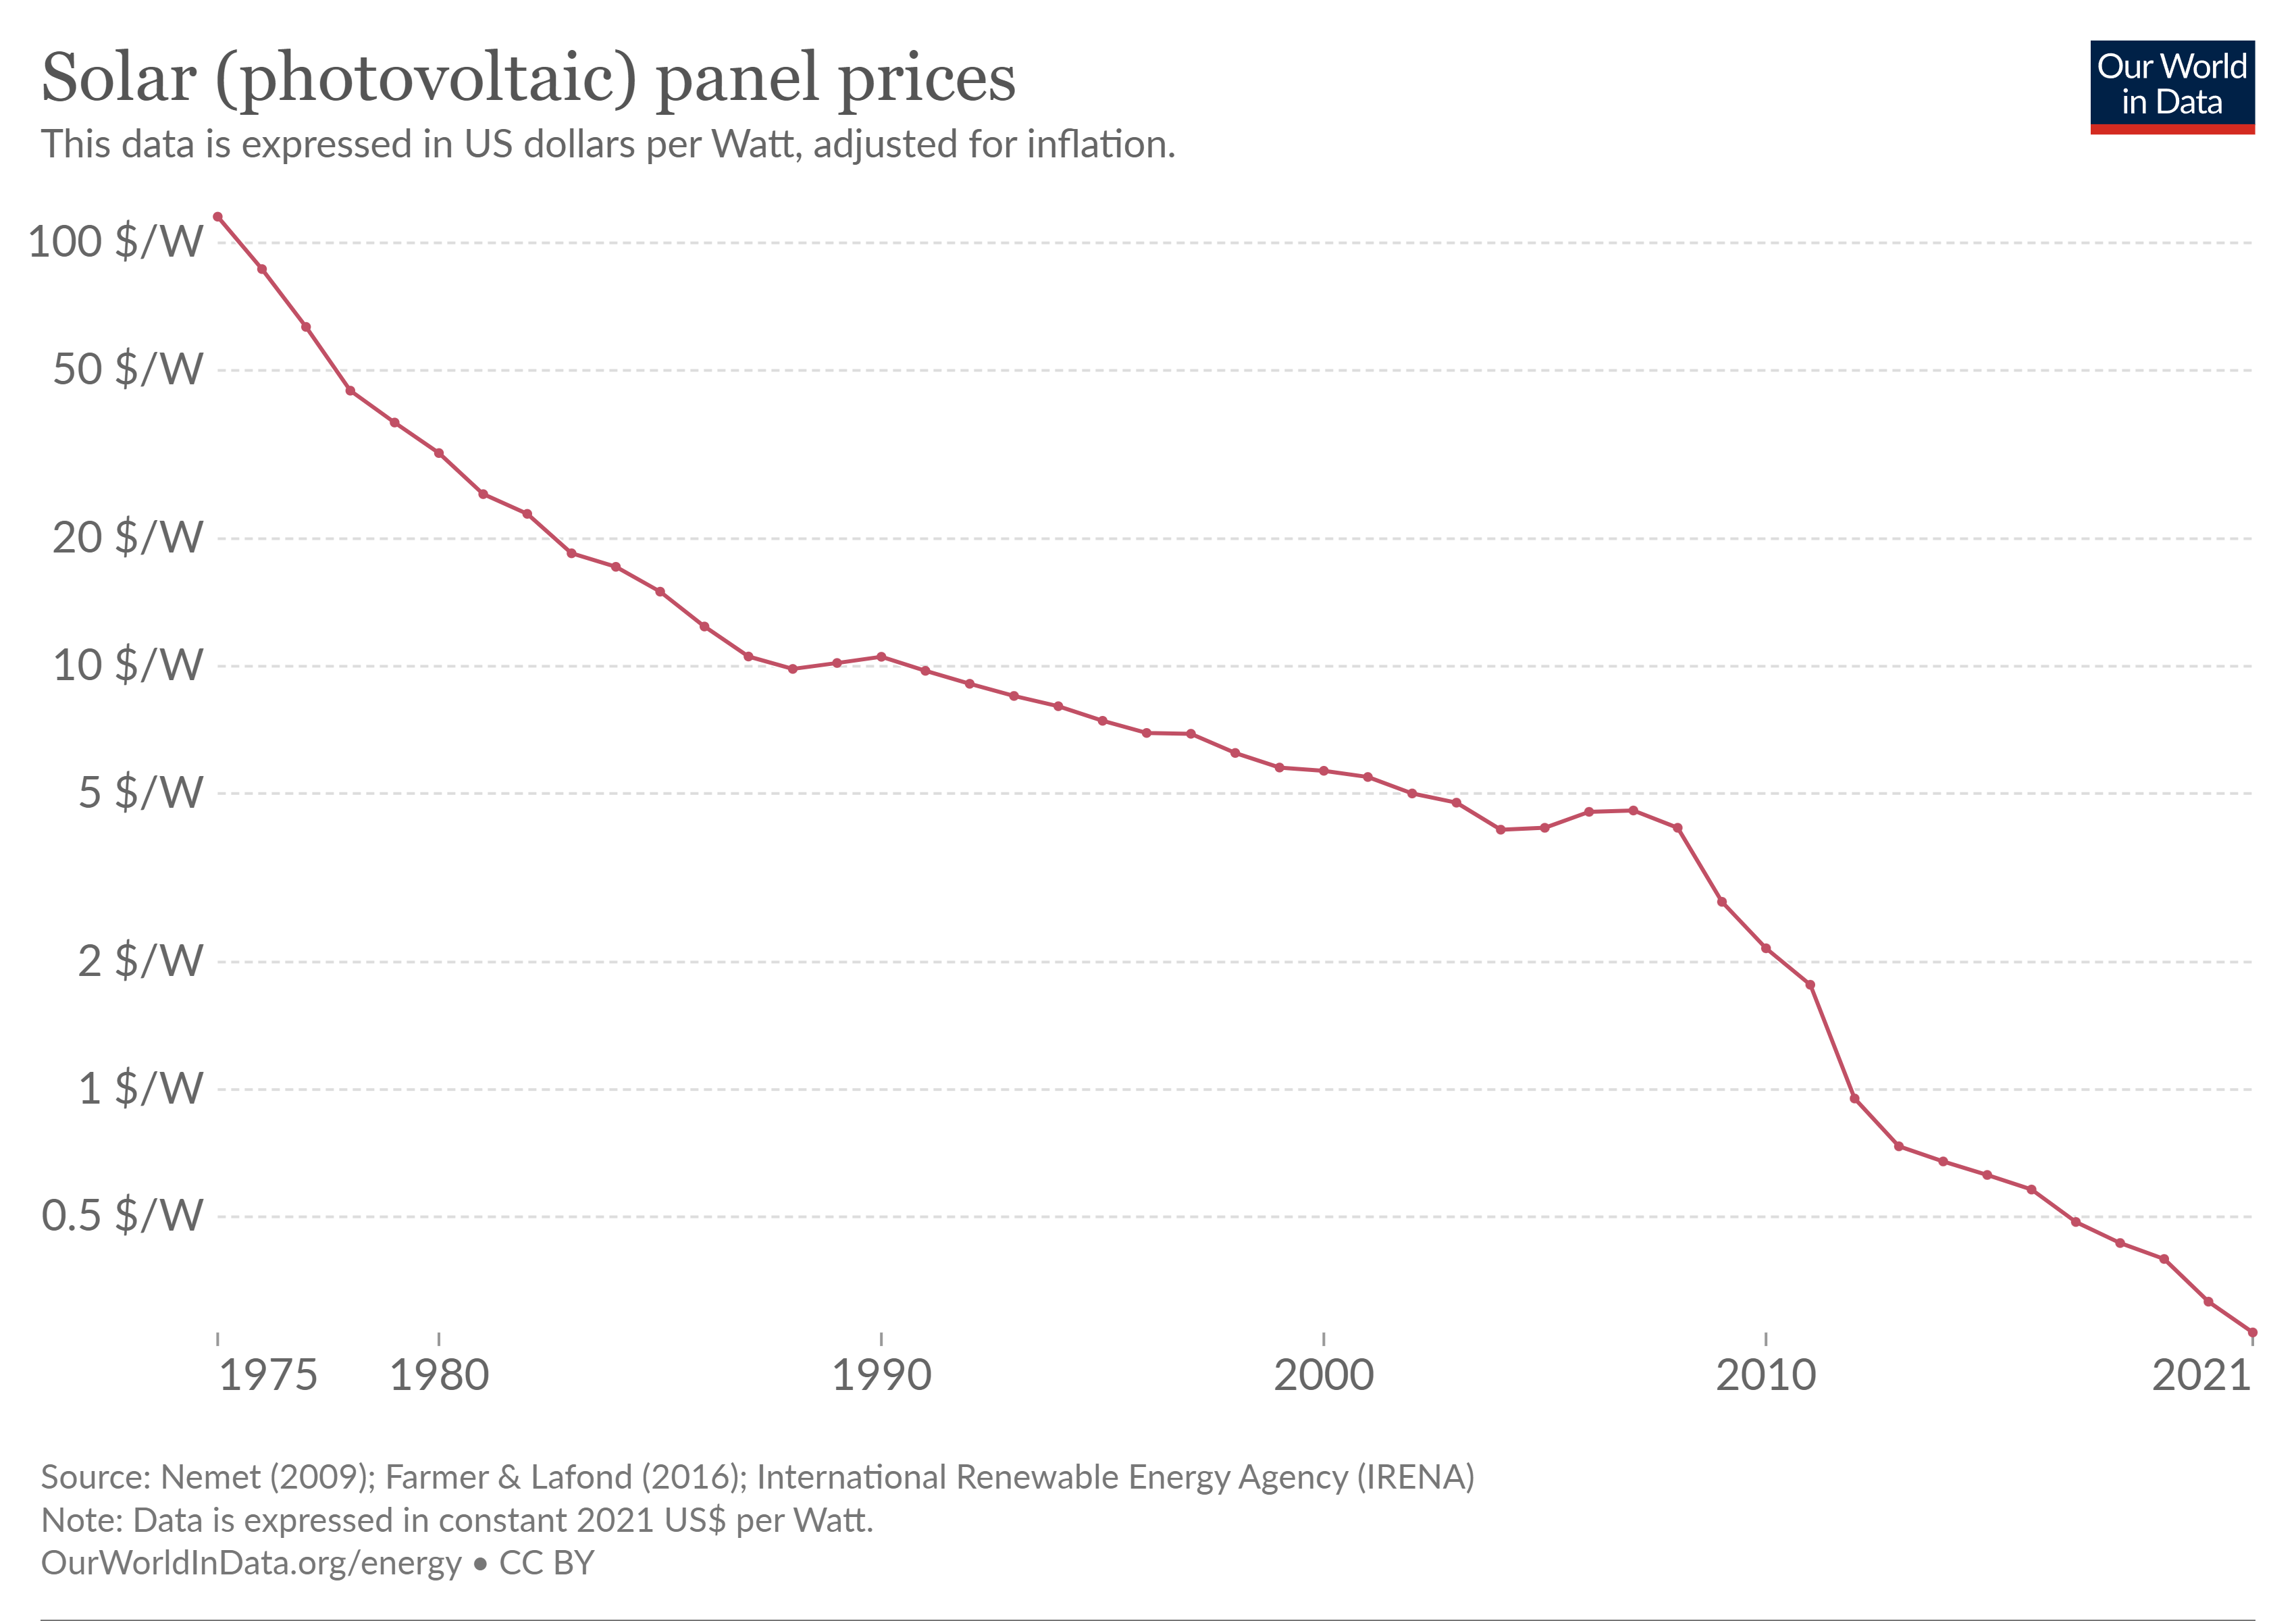
\includegraphics[width=0.7\linewidth]{images/solar-pv-prices.png}
    \caption{Decline in Solar Panel Prices Over the Past Decade \cite{irena}}
    \label{fig:solar_panel_prices}
\end{figure}
\noindent The graph in Figure \ref{fig:solar_panel_prices} illustrates the notable decline in solar panel prices over the past decades, making solar energy systems increasingly
cost-effective.
Solar energy production requires substantial land or rooftop space for photovoltaic installations, which in densely populated regions
like Germany necessitates careful planning and consideration of competing land uses.

\section*{Data \& Modeling}
To maximize the efficiency of solar power generation, it is crucial to optimize the orientation of solar panels.
\\~\\
During Ferienakademie we prototyped the Solar Power Estimator, a tool designed to estimate the solar power generated by a system over a period of time and to optimize the orientation of solar panels.
The tool utelizes satellite data from the European Union and the Python library pvlib for accurate panel array modeling \cite{F.Holmgren.2018}.
\subsection*{Data}
To start, the tool fetches radiation data from the photovoltaic geographical information system (PVGIS) \cite{EnergyDGJointResearchCentre.2016}, which given latitude and longitude
can return very accurate radiation data from 2005 to 2020. Moreover, the radiation is already split into direct, diffuse and reflected radiation. The data is computed from satellite data, which makes it 
extremely accurate and can serve as a very good average to plan a future solar power plant. Furthermore the californa energy commission allows access to their extensive module database \cite{.02.10.2023} for over
20,000 panels and a lot of inverters. As quality of life feature, the tool uses the maptiler \cite{MapTilerAG.26.09.2023} and mapbox \cite{.02.10.2023b} services for geocoding and map rendering.
The remaining parameters such as simulation time, house height, roof tilt, roof azimuth, panel tilt, panel azimuth, number of modules, module type, inverter type and casing have to be specified by the user,
some of those from presets provided by pvlib.
\subsection*{Modeling}
The simulation begins with the irradtion data provided by PVGIS, which requires two calls since pvlib requires the direct normal irradiance ($dni$), the diffuse horizontal irradiance ($dhi$) 
and the global horizontal irradiance ($ghi$) and we can only fetch data for a tracked panel resulting in a constantly normal panel and a tilted panel. In addition, air temperature and wind speed is provided.
With this information pvlib firstly estimate the solar position, airmass, albedo and angle of incidence for a fixed panel, which is the only one our tool supports thus far. From those estimations the total irradiance
is calculated. This can be further modified by an AOI model for moving panels and optionally a spectral model, which results in an effective irradiance. With this information the tool uses the respective module and
casing models to calculate the DC output of the panel, with respect to effective irradiance and cell temperature. The DC outputs of the panels are aggregated and then converted to AC output by the inverter model.
\\~\\
For comparison Figure \ref{fig:comparison} shows the initial pipeline concipated in preparation for Ferienakademie and the final one now in use. One can see that the pipeline reaches further but is also reduced in complexity
by the usage of pvlib. 
\begin{figure}[H]
    \centering
    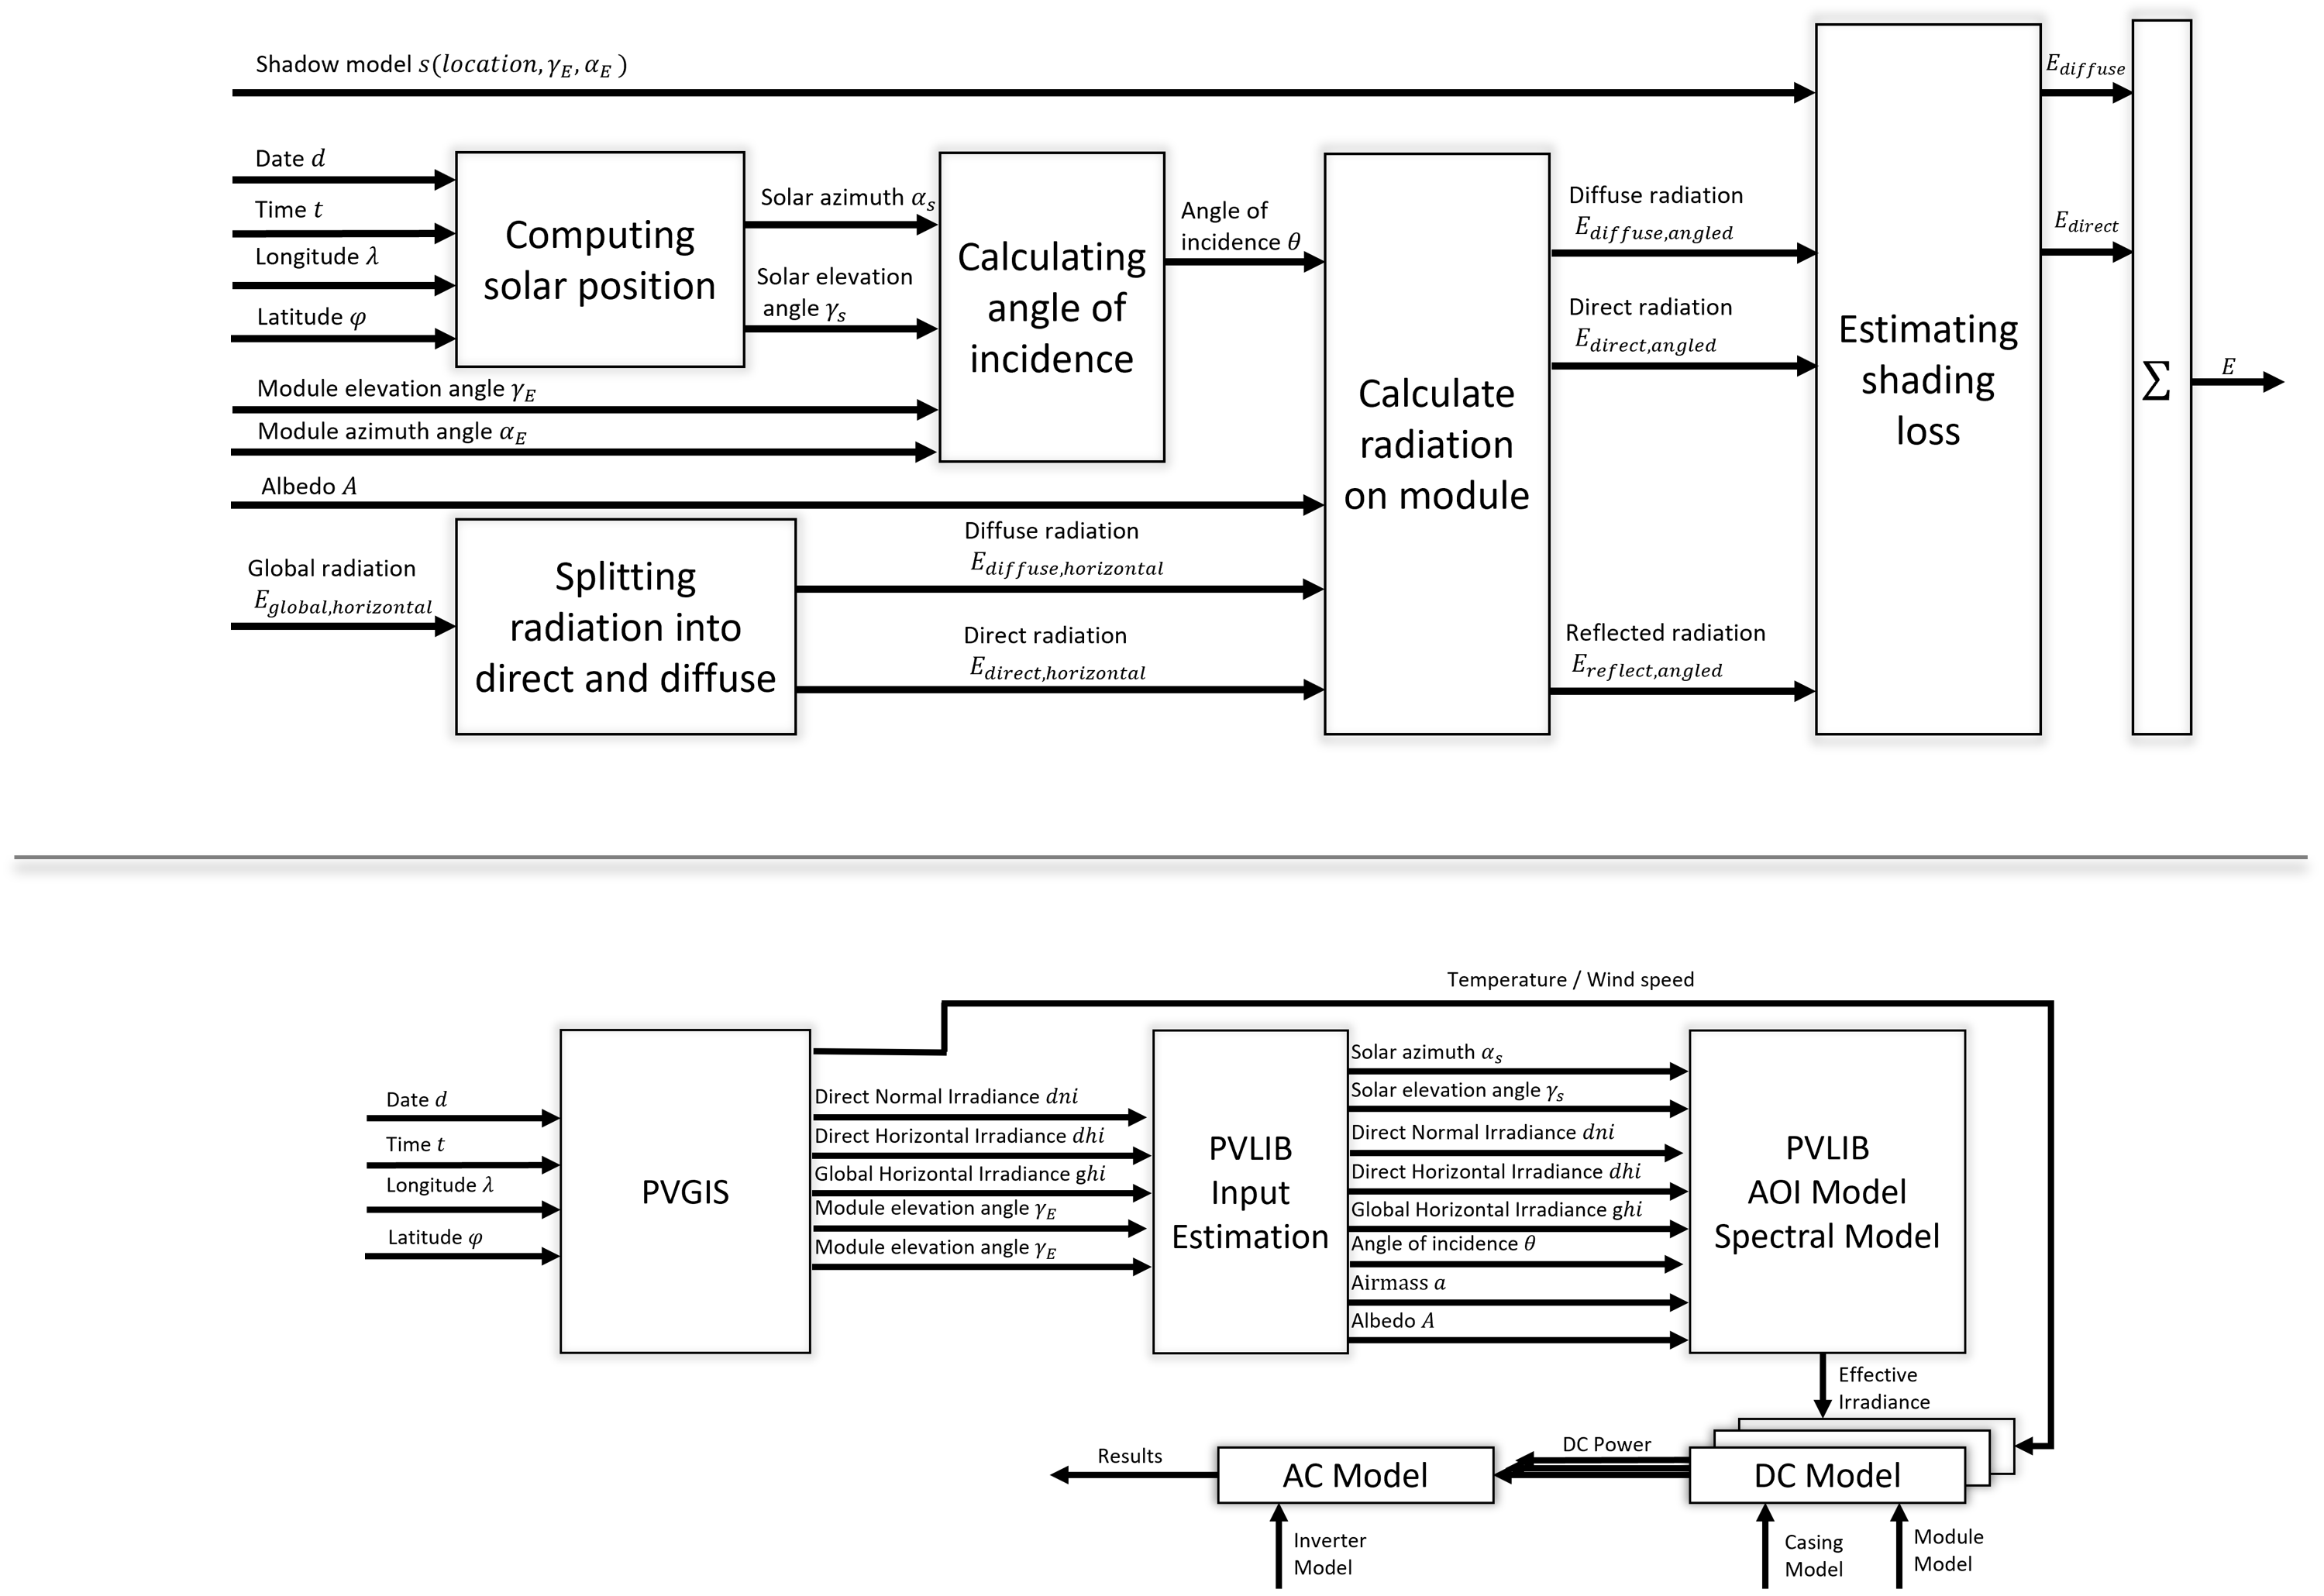
\includegraphics[width=1.0\linewidth]{images/comparison.png}
    \caption{Comparison of concepts before and after Ferienakademie}
    \label{fig:comparison}
\end{figure}

\section*{Optimization}
While the entire pipeline is in principle differentiable, our heavy usage of library code made it impossible to use automatic differentiation, which lead us to abstain from any gradient-based optimization
techniques since manual differentiation and reimplementation was deemed to time consuming. \\Furthermore, the optimization of tilt and azimuth angle did not have to be very accurate only to about 1° 
and was heavily constraint (for tilt [roof-tilt, 90°], for azimuth angle [0, 360°]). Therefore, it seemed feasible to use a blackbox optimization algorithm,
which does not require any gradient information. The algorithm of choice was the Nelder-Mead \cite{.1965} algorithm, as implemented in the scipy library, while this one obviously converged slower than
gradient-based methods, and neither gives any convergence guaranetess, it seemed to converge quite robustly in our case, always giving reasonable power output improvements,
and using about 50 function evaluations.
\section*{Dashboard}
\begin{figure}[H]
    \centering
    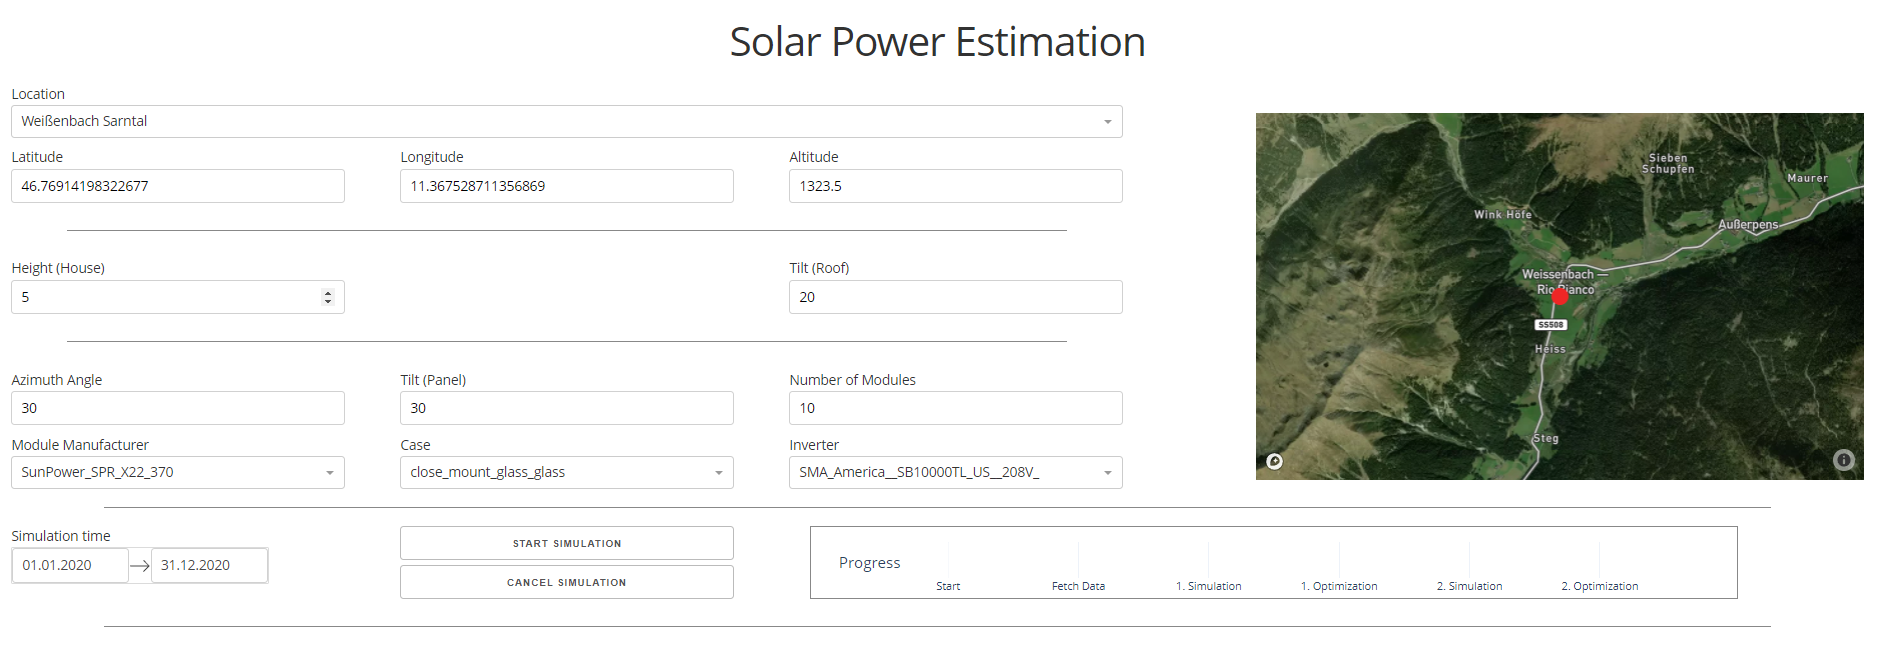
\includegraphics[width=1.0\linewidth]{images/dashboard_input.PNG}
    \caption{Dashboard input}
    \label{fig:input}
\end{figure}
\noindent For our dashboard the python library dash-plotly \cite{.02.10.2023c} was used, which creates html and javascript code automatically from the specifications in python.
This way the entire project could be coded in python. The dashboard is split into two parts, the input and the result section.
\\~\\
The input section is shown in Figure \ref{fig:input} and is further split into several regions. In the first region the user specifies the location of the solar power plant. This can be done by either entering the
coordinates directly or by utilizing the search bar, which geocodes the given name. The second region is used to specify the house parameters, namely the height and roof tilt.
Thirdly, the photovoltaic parameters are specified, such as the azimuth angle and tilt of the panels, the number of modules and which module, casing and inverter to use. 
The last section is used to specify the simulation time and shows a progress bar for the at times lengthy simulation.
\\~\\
\begin{figure}[H]
    \centering
    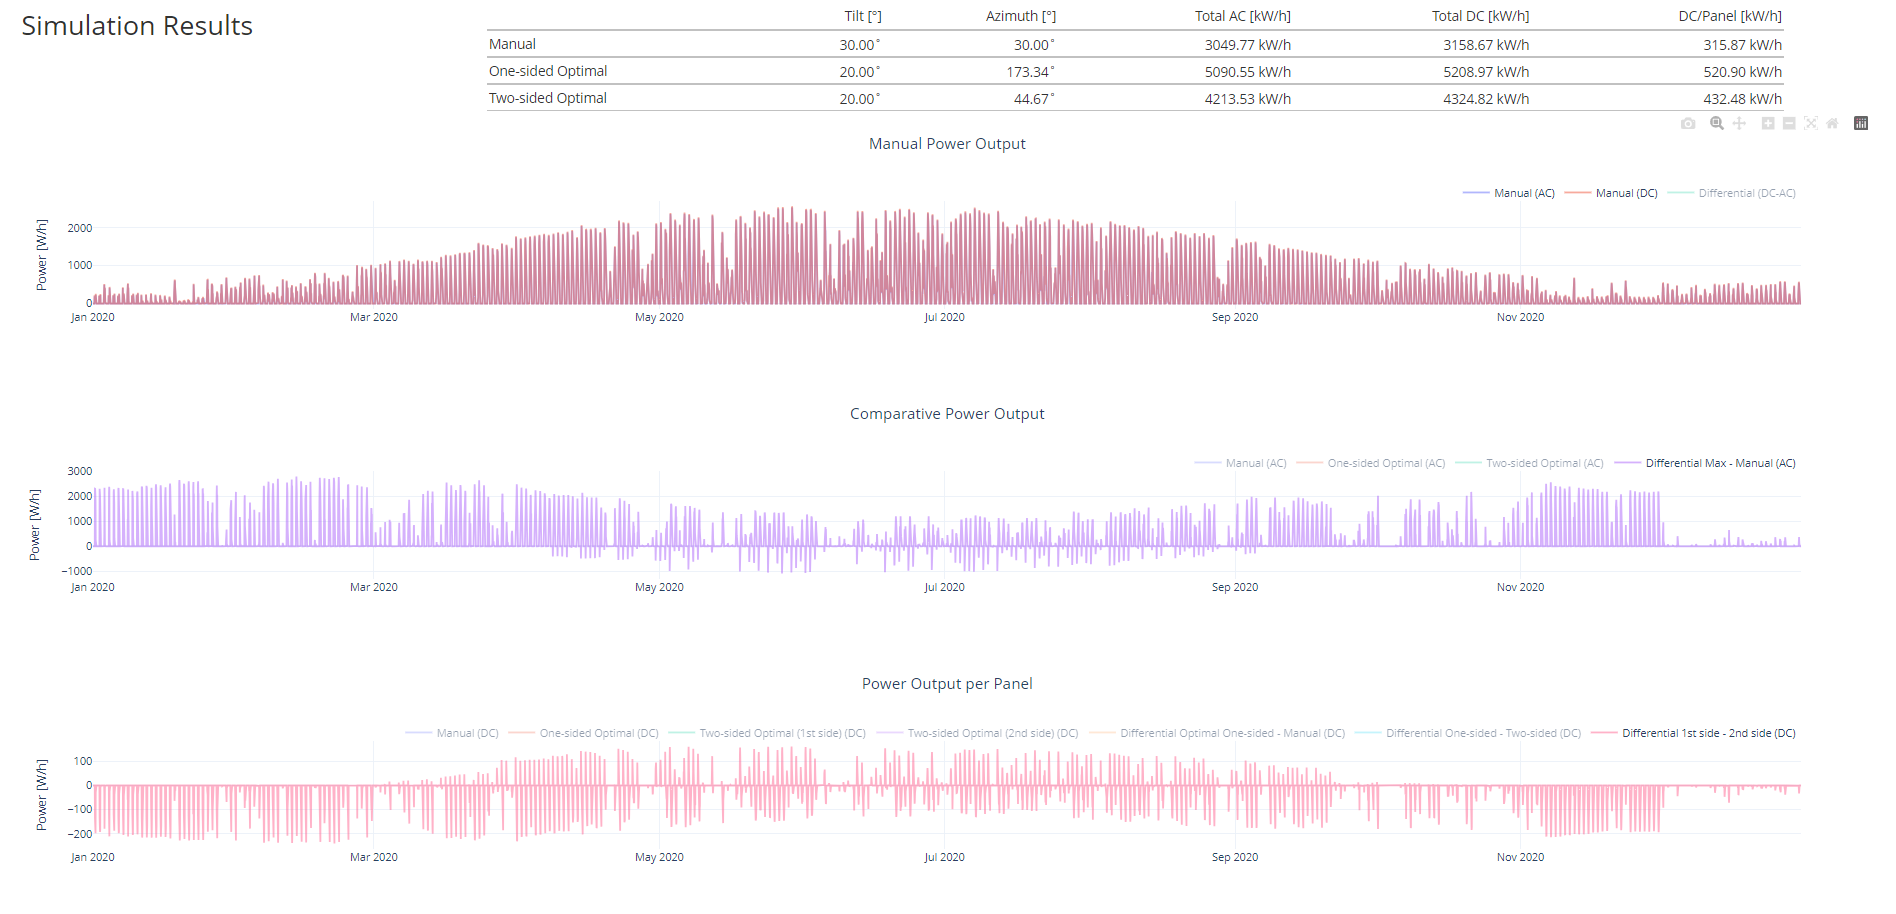
\includegraphics[width=1.0\linewidth]{images/dashboard_output.PNG}
    \caption{Dashboard input}
    \label{fig:output}
\end{figure}

\noindent The output section is shown in Figure \ref{fig:output} and consists of a data table, where the most important numbers are displayed, and three plots.
The first plot shows the difference between the AC and DC output of the system, which helps to spot poor inverter choices. The second plot shows comparisons between the manual
setup and the optimized setups to visualize during which times an optimized system would outperform the given.
The last plot compares the DC output per panel of the various simulated systems, which is a more direct measure of how much irradiance the panels receive dependening on their orientation.
\section*{Shortcomings}
While we were quite content with the accuracy and speed of the tool, especially given the limited development time, there are still various shortcomings
that have to be addressed in the future. Firstly, the tool estimates some factors very roughly, for example the albedo of the surroundings and more importantly the shadow cast by the surrounding landscape.
More pressing, however is the lack of an optimization
for a given azimuth angle, since so far the azimuth angle is changed arbitrarily by the optimization. Furthermore, the tool does not support rotating modules and could also be enhanced in terms of 
simulation speed. One bug, that was actually fixed after Ferienakademie, was the wrong incorporation of the weather data, which resulted in a less significant difference between the different tilt
and azimuth angles. In the future, I might continue to fix the mentioned shortcomings and get a precision estimate by comparing it to real world data.


\bibliography{citavi}
\bibliographystyle{ieeetr}
\end{document}